%\documentclass[review]{elsarticle}
\documentclass[final,5p,times,twocolumn]{elsarticle}

\usepackage[english]{babel}
\usepackage[utf8]{inputenc}
\usepackage{amsmath}
\usepackage{graphicx}
\usepackage[colorinlistoftodos]{todonotes}
\usepackage{hyperref}
\usepackage{soul}
\usepackage{algorithm}
\usepackage{algorithmic}
\usepackage{makeidx}  % allows for indexgeneration
\usepackage[section]{placeins}
\usepackage{float}

%\modulolinenumbers[5]


% Commands
\newcommand{\note}[2][inline]{\todo[color=yellow!30,#1]{\small\sf #2}}
\newcommand{\comment}[2][inline]{\todo[color=red!30,#1]{\small\sf #2}}

\journal{Future Generation Computer Systems}

\begin{document}
\begin{frontmatter}

% Title
\title{A Semantic-Based Approach to Attain Reproducibility of Computational Environments in Scientific Workflows: A Case Study}

% Authors and Institutions
\author[upm]{Idafen Santana-Perez\corref{cor1}}
\ead{isantana@fi.upm.es}

\author[isi]{Rafael Ferreira da Silva}
\ead{rafsilva@isi.edu}

\author[isi]{Mats Rynge}
\ead{rynge@isi.edu}

\author[isi]{Ewa Deelman}
\ead{deelman@isi.edu}

\author[upm]{Mar\'ia~S.~P\'erez-Hern\'andez}
\ead{mperez@fi.upm.es}

\author[upm]{Oscar Corcho}
\ead{ocorcho@fi.upm.es}

\cortext[cor1]{Corresponding address: Ontology Engineering Group (OEG), Laboratorio de Inteligencia Artificial, Facultad de Inform\'atica, Universidad Polit\'ecnica de Madrid, Avda. Montepr\'incipe, s/n, Boadilla del Monte, 28660, Spain}

\address[upm]{Ontology Engineering Group, Universidad Polit\'ecnica de Madrid, Madrid, Spain }
\address[isi]{University of Southern California, Information Sciences Institute, Marina del Rey, CA, USA}


% Abstract
\begin{abstract}
Reproducible research in scientific workflows is often addressed by tracking the provenance of the produced results. While this approach allows inspecting intermediate and final results, improves understanding, and permits replaying a workflow execution, it does not ensure that the computational environment is available for subsequent executions to reproduce the experiment. In this work, we propose describing the resources involved in the execution of an experiment using a set of semantic vocabularies, so as to conserve the computational environment. We define a process for documenting the workflow application, management system, and their dependencies based on 4 domain ontologies. We then conduct an experimental evaluation using a real workflow application on an academic and a public Cloud platform. Results show that our approach can reproduce an equivalent execution environment of a predefined virtual machine image on both computing platforms.
\end{abstract}

\begin{keyword}
Semantic Metadata \sep Scientific Workflow \sep Reproducibility
\end{keyword}


\end{frontmatter}


% Introduction
\section{Introduction}

Reproducibility of results of published scientific experiments is a cornerstone in science. Therefore, the scientific community has been encouraging researchers to publish their contributions in a verifiable and understandable way~\cite{YaleRoundtable09}. 
In computational science, or \emph{in-silico} science, reproducibility often requires that researchers make code and data publicly available so that the data can be analyzed in a similar manner as in the original work described in the publication. Code must be available to be distributed, and data must be accessible in a readable format~\cite{bookReproducibility}. 

In the context of scientific experiments, terms such as reproducibility, replicability, and repeatability are sometimes used as synonymous. Even though there is no clear consensus on how to define both (definitions may vary over different scientific areas), in this work we understand them as separated concepts~\cite{Drummond2011}. In this work, we address the reproducibility of the execution environment for a scientific workflow, as we do not aim to obtain an exact incarnation of the original one, but rather an environment that is able to support the required capabilities exposed by the former environment.

Scientific workflows are a useful representation for managing the execution of large-scale computations. Many scientists now formulate their computational problems as scientific workflows running on distributed computing infrastructures such as campus Clusters, Clouds, and Grids~\cite{workflowBook}. This representation not only facilitates the creation and management of the computation but also builds a foundation upon which results can be validated and shared. Since workflows formally describe the sequence of computational and data management tasks, it is easy to trace the origin of the data produced. Many workflow systems capture provenance at runtime, which provides the lineage of data products and as such underpins the whole of scientific data reuse by providing the basis on which trust and understanding are built. A scientist would be able to look at the workflow and provenance data, retrace the steps, and arrive at the same data products. 
However, this information is not sufficient for achieving full reproducibility.

Currently, most of the approaches in computational science conservation, in particular for scientific workflow executions, have been focused on data, code, and the workflow description, but not on the underlying infrastructure---which is composed of a set of computational resources (e.g. execution nodes, storage devices, and networking) and software components. We identify two approaches for conserving the environment of an experiment: \emph{physical conservation}, where the real object is conserved due to its relevance and the difficulty in obtaining a counterpart; and \emph{logical conservation}, where objects are described in such a way that an equivalent one can be obtained in a future experiment.

The computational environment is often conserved by using the physical approach, where computational resources are made available to scientists over a sustained period of time. As a result, scientists are able to reproduce their experiments in the same environment. However, such infrastructures demand huge maintenance efforts, and there is no guarantee that it will not change or suffer from a natural decay process~\cite{Gavish2011637}. Furthermore, the infrastructure may be subjected to organization policies, which restricts its access to a selective group of scientists, thus limiting reproducibility to this restricted group. On the other hand, data, code, and workflow description can be conserved by using a logical approach that is not subjected to natural decay processes. 

Accordingly, we propose a logical-oriented approach to conserve computational environments, where the capabilities of the resources (virtual machines (VM)) are described. From this description, any scientist, interested in reproducing an experiment, will be able to reconstruct the former infrastructure (or an equivalent one) in any Cloud computing infrastructure (either private or public). One may argue that it would be easier to keep and share VM images with the community research through a common repository, however the high storage demand of VM images remains a challenging problem~\cite{Mao:2014:ROD:2600090.2512348,6552826}. 

Our approach uses semantic-annotated workflow descriptions to generate lightweight scripts for an experiment management API that can reconstruct the required infrastructure. We propose to describe the resources involved in the execution of the experiment, using a set of semantic vocabularies, and use those descriptions to define the infrastructure specification. This specification can then be used to derive the set of instructions that can be executed to obtain a new equivalent infrastructure. We conduct a practical evaluation for a real scientific workflow application in which we describe the application and its environment using a set of semantic models, and use an experiment management tool to reproduce a workflow execution in two different Cloud platforms. 

In this work we entail reproducibility from the execution environment point of view. For  the sake of showing how our approach works, we provide an example in which we have also include the data and the workflow execution of the experiment.

The paper is organized as follows. Section~\ref{sec:semantic} describes our semantic approach for documenting computational infrastructures. Section~\ref{sec:reproducibility} presents the practical evaluation and the description of the tools used to implement the semantic models and manage the experiment. Section~\ref{sec:related-work} presents the related work, and Section~\ref{sec:conclusion} summarizes our results and identifies future works.



% Section: Semantic Modeling
\section{Semantic Modeling of Computational Resources}
\label{sec:semantic}

Scientific workflows are also used for preserving and sharing scientific experiments in science. Research efforts focused on describing the workflow structure and the experimental data, both input data and results.
In this work, we argue that the information about the computational resources should be also provided for achieving full reproducibility. 
These descriptions  allow the target audience, usually another scientist in the same domain, to understand the underlying components involved in a workflow execution.

We propose the definition of semantic models for describing the main domains of a computational infrastructure, and for defining the taxonomy of concepts and the relationships between them. These models describe the software components, hardware specifications, and the available computational resources (in the form of VMs). They also capture infrastructure dependencies of the workflows. As a result, this process facilitates experiment's reusability since a new experiment, which may reuse parts of the workflow previously modeled, or a reproduction of a workflow, would benefit from the infrastructure dependencies already described.

We have identified four main domains of interest for documenting computational scientific infrastructures. We have developed a set of models, one for each domain, and an ontology network that defines the inter-domain relations between these models (Figure~\ref{fig:wicusrels}):

\begin{itemize}
	\setlength{\itemsep}{1pt}
    \setlength{\parskip}{0pt}
    \setlength{\parsep}{0pt}

	\item{\emph{Hardware domain}}: identifies the most common hardware information, including CPU, Storage and RAM memory, and their capacities.
	
    \item{\emph{Software domain}}: defines the software components involved on the execution. It includes the pieces of executable software (e.g. scripts, binaries, and libraries) used in the experiment. In addition, dependencies between those components and configuration information are also defined, as well as the required steps for deploying them.
	
    \item{\emph{Workflow domain}}: describes and relates workflow fragments (a.k.a transformations) to their dependencies. Therefore, scientists can understand what are the relevant infrastructure components for each part of the workflow.
	
    \item{\emph{Computing Resources domain}}: expresses the information about the available computing resources. In this domain, only virtualized resources are currently considered (i.e. VMs). It includes the description of the VM image, its provider, and specifications.
\end{itemize}

\begin{figure}[!htb]
	\centering
    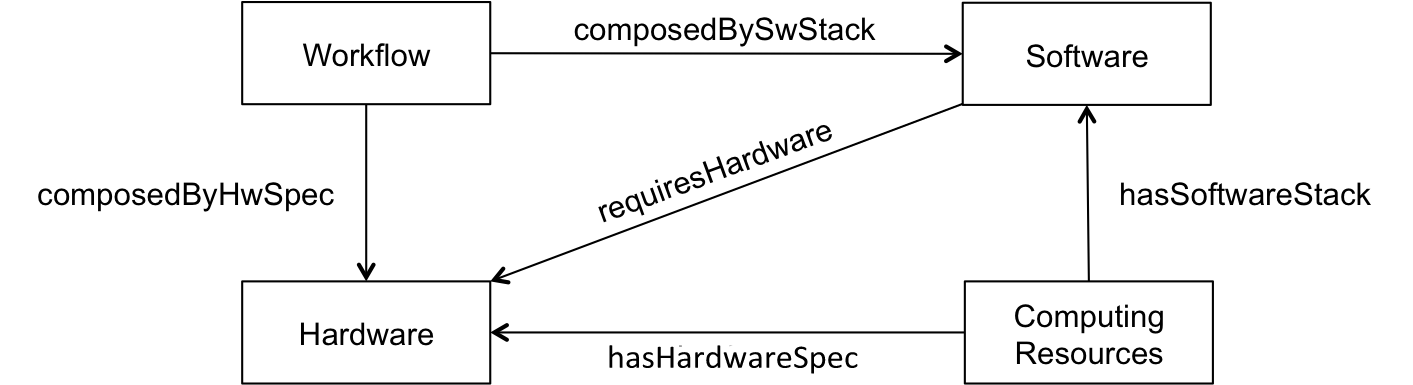
\includegraphics[width=\linewidth]{figures/wicusrels}
    \caption{Overview of the ontology network ($\rightarrow$ denotes inter-domain relation).}
    \label{fig:wicusrels}
\end{figure}



% Section
\section{Reproducibility in Scientific Workflows}
\label{sec:reproducibility}

In this section, we conduct a practical evaluation through experimentation in which we instantiate the semantic models aforementioned for a real scientific workflow application. We study and document the Montage~\cite{Montage} workflow and its execution environment, which includes the application software components and the workflow management system. Montage is and astronomy workflow application that is widely used by many astronomers to construct large image mosaics of the sky.


\subsection{Scientific Workflow Execution}

In this work, we use the Pegasus WMS~\cite{Pegasus, Deelman-FGCS-2014} as our workflow engine. The Pegasus WMS can manage workflows comprised of millions of tasks, recording data about the execution and intermediate results. In Pegasus, workflows are described an abstract workflows, which do not contain resource information, or the physical locations of data and executables. The abstract workflow description is represented as a DAX (DAG in XML), capturing all the tasks that perform computation, the execution order of these tasks, and for each task the required inputs, expected outputs, and the arguments with which the task should be invoked. During a workflow execution, the Pegasus WMS translates an abstract workflow into an executable workflow, determining the executables, data, and computational resources required for the execution.
Pegasus maps executables to their installation paths or to a repository of stageable binaries defined in a Transformation Catalog (TC).
A workflow execution includes data management, monitoring, and failure handling. Individual workflow tasks are managed by a task scheduler (HTCondor~\cite{condor}), which supervises their execution on local and remote resources.


\subsection{Reproducibility Tools}

To conduct the experimental evaluation, we use the WICUS framework, which comprises the semantic models described in Section~\ref{sec:semantic} and a set of tools for annotating and consuming data, and the PRECIP~\cite{Azarnoosh-CRC-2013} experiment management tool to manage the experiment. Below, we describe each of these tools in detail.


\subsubsection{WICUS.}
We introduce here the Workflow Infrastructure Conservation Using Semantics ontology (WICUS), an OWL2~\cite{OWL2} (Web Ontology Language) ontology network that implements the semantic models introduced in Section~\ref{sec:semantic}. This ontology network is available online\footnote{\url{http://purl.org/net/wicus}} and it is a continuous effort to discover and define the relevant and required properties for describing scientific computational infrastructures. 

Besides the ontology network, WICUS has a set of modules that facilitates the annotation of the resources involved on the execution of a scientific workflow. These tools are not fully automated yet, but represent a first step on helping users to define the requirements of their experiments. Figure~\ref{fig:wicusflow} shows the main modules, their flow and intermediate results involved in the process for achieving reproducibility, and describes the process of data generation and consumption.

\begin{figure}[!htb]
	\centering
	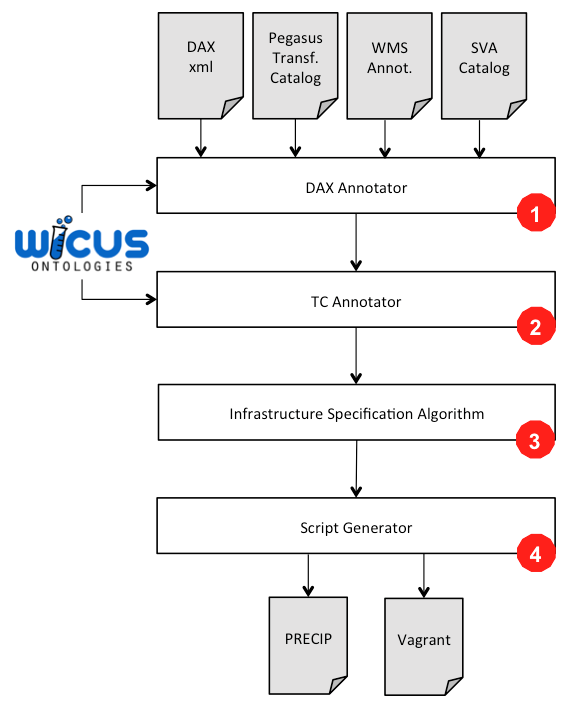
\includegraphics[width=\linewidth]{figures/wicusflow}
	\caption{WICUS annotation modules and flow.}
	\label{fig:wicusflow}
\end{figure}

\noindent \textbf{1. DAX Annotator.} This tool parses a DAX (Pegasus' workflow description) and generates a set of annotations, using the terms of the WICUS vocabulary, representing workflow transformations and the workflow infrastructure requirements.

\noindent \textbf{2. Workflow annotations.} An RDF file containing the description of the workflow and its infrastructure requirements.

\noindent \textbf{3. WMS annotations.} An RDF file containing the information of the WMS component and its dependencies. This information will be added to the Software Components Catalog.

\noindent \textbf{4. Transformation Catalog Annotator.} This tool parses the Pegasus Transformation Catalog (which describes the binaries involved on the workflow execution and their locations) and the WMS annotations file, to generate two set of annotations: the \emph{Software Components Catalog} and the \emph{Workflow \& Configuration Annotation} files.

\noindent \textbf{5. Software Components Catalog.} An RDF file containing the set of annotations about the binaries, dependencies, deployment plans and scripts, and configuration information of the software involved in the experiment.

\noindent \textbf{6. Workflow \& Configuration Annotation File.} An RDF file containing the same information as in 2, but enriched with the configuration information for each workflow execution step, as specified in the transformation catalog.

\noindent \textbf{7. Scientific Virtual Appliances Catalog.} An RDF file describing available VM appliances. Information about the related infrastructure providers and the VM images that compose an appliance are included in this dataset.

\noindent \textbf{8. Infrastructure Specification Algorithm.} This process reads files 5, 6, and 7, and generates a configuration file (e.g. a PRECIP script), which describes VMs and software components to be created and deployed.

\noindent \textbf{9. PRECIP script.} This script creates a PRECIP experiment, which runs a VM, copies the required binaries, and executes deployment scripts to set the environment for the workflow execution. It also contains the PRECIP commands from the original experiment in order to re-execute it.


\subsubsection{PRECIP.}
The Pegasus Repeatable Experiments for the Cloud in Python (PRECIP)~\cite{Azarnoosh-CRC-2013} is a flexible experiment management control API for running experiments on all types of Clouds, including academic Clouds such as FutureGrid~\cite{futuregrid}, and commercial Clouds such as Amazon EC2~\cite{aws}. In PRECIP, interactions with the provisioned instances are done by tagging. When an instance is provisioned, the scientist can add arbitrary tags to that instance in order to identify and group the instances in the experiment. API methods such as running remote commands, or copying files, all use tags to specify which instances to target. PRECIP does not force the scientist to use a special VM image, and no PRECIP components need to be pre-installed in the image. Scientists can use any basic Linux image and PRECIP will bootstrap instances using SCP and SSH commands. PRECIP provides functionality to run user-defined scripts on the instances to install/configure software and run experiments, and also manages SSH keys and security groups automatically.

In this work, PRECIP usage is twofold. First, the tool is used to describe and perform a workflow execution using the Pegasus WMS on a predefined VM image. Second, the WICUS annotation modules use PRECIP to generate a script able to reproduce the execution environment of the former experiment, and run it on different Cloud platforms.



\subsection{Experimental Evaluation}

The goal of this experiment is to reproduce an original workflow execution in two different Cloud infrastructures: FutureGrid~\cite{futuregrid} and Amazon EC2~\cite{aws}. FutureGrid is an academic Cloud test-bed facility that includes a number of computational resources at distributed locations. Amazon Web Services EC2 is a public infrastructure provider and the \emph{de facto} standard for IaaS Cloud platforms.


\subsubsection{Scientific Workflows}

\paragraph{\textbf{Montage}}
The Montage workflow~\cite{Montage} was created by the NASA Infrared Processing and Analysis
Center (IPAC) as an open source toolkit that can be used to generate custom mosaics of
astronomical images in the Flexible Image Transport System (FITS) format. In a Montage workflow,
the geometry of the output mosaic is calculated from the 
input images. The inputs are then re-projected to have the same spatial scale and rotation, 
the background emissions in the images are corrected to have a uniform level, and the 
re-projected, corrected images are co-added to form the output mosaic.
Figure~\ref{fig:workflow-montage} illustrates a small (20 node) Montage workflow. 
The size of the workflow depends on the number of images required to construct the 
desired mosaic. The workflow instances used in this paper generate 2, 4, or 8 degree square
mosaics using 275, 840, and 2640 input images from the 2 Micron All Sky Survey (2MASS).

\begin{figure}[!htt]
	\centering
	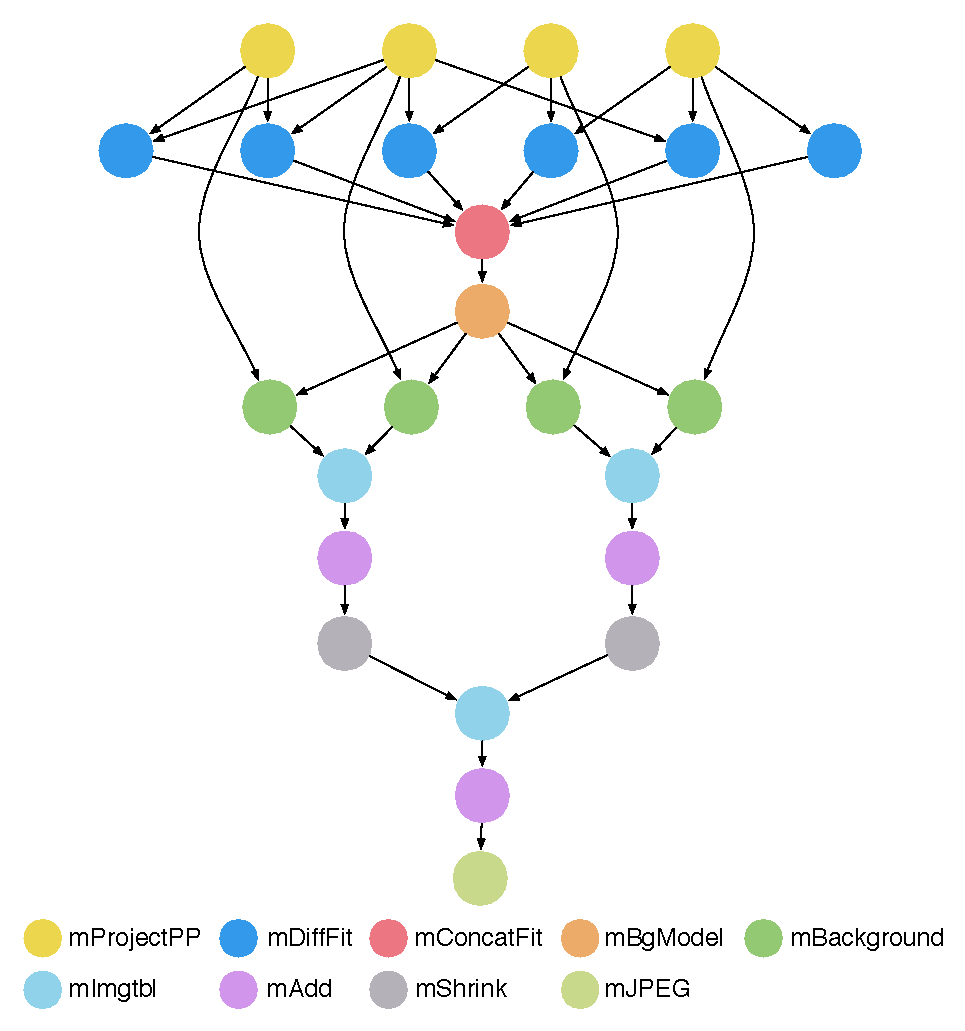
\includegraphics[width=0.9\linewidth]{figures/workflow-montage}
	\caption{A small (20 node) Montage workflow.}
	\label{fig:workflow-montage}
\end{figure}


\paragraph{\textbf{Epigenomics}}
The USC Epigenome Center~\cite{genome} is currently involved in mapping the epigenetic 
state of human cells on a genome-wide scale. The Epigenomics workflow 
(Figure~\ref{fig:workflow-genome}) processes multiple sets of genome sequences in
parallel. These sequences are split into subsets, the subsets are filtered to remove
contaminants, reformatted, then mapped to a reference genome. The mapped sequences are
finally merged and indexed for later analysis. In this paper, the Epigenome
workflow was used to align 13 million genome sequence reads to a reference genome
for human chromosome 21. The size of the workflow depends on the 
chunking factor used on the input data (\texttt{binsize}), which determines
the number of sequence reads in each chunk.

\begin{figure}[!htb]
	\centering
	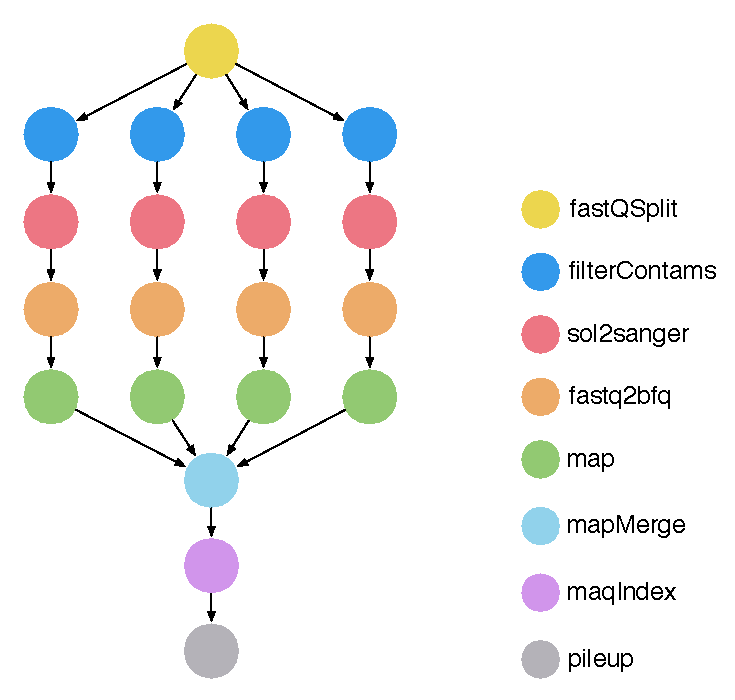
\includegraphics[width=0.75\linewidth]{figures/workflow-genome}
	\caption{Epigenomics workflow.}
	\label{fig:workflow-genome}
\end{figure}

\paragraph{\textbf{SoyKB}}
The SoyKB workflow~\cite{soybean, Joshi01012014} is a genomics pipeline 
that re-sequences soybean germplasm lines selected for desirable traits such 
as oil, protein, soybean cyst nematode resistance, stress resistance, and root 
system architecture. The workflow (Figure~\ref{fig:workflow-soykb}) 
implements a SNP and injection/deletion (indel) identification and analysis 
pipeline using the GATK haplotype caller~\cite{gatk} and a soybean reference 
genome. The workflow analyzes samples in parallel to align them to the reference 
genome, to de-duplicate the data, to identify indels and SNPs, and to merge and 
filter the results. The results are then used for genome-wide association studies 
(GWAS) and genotype to phenotype analysis. The workflow instance used in this 
paper is based on a sample dataset of 50 sequence reads that requires less 
memory than a full-scale production workflow.

\begin{figure}[!htb]
	\centering
	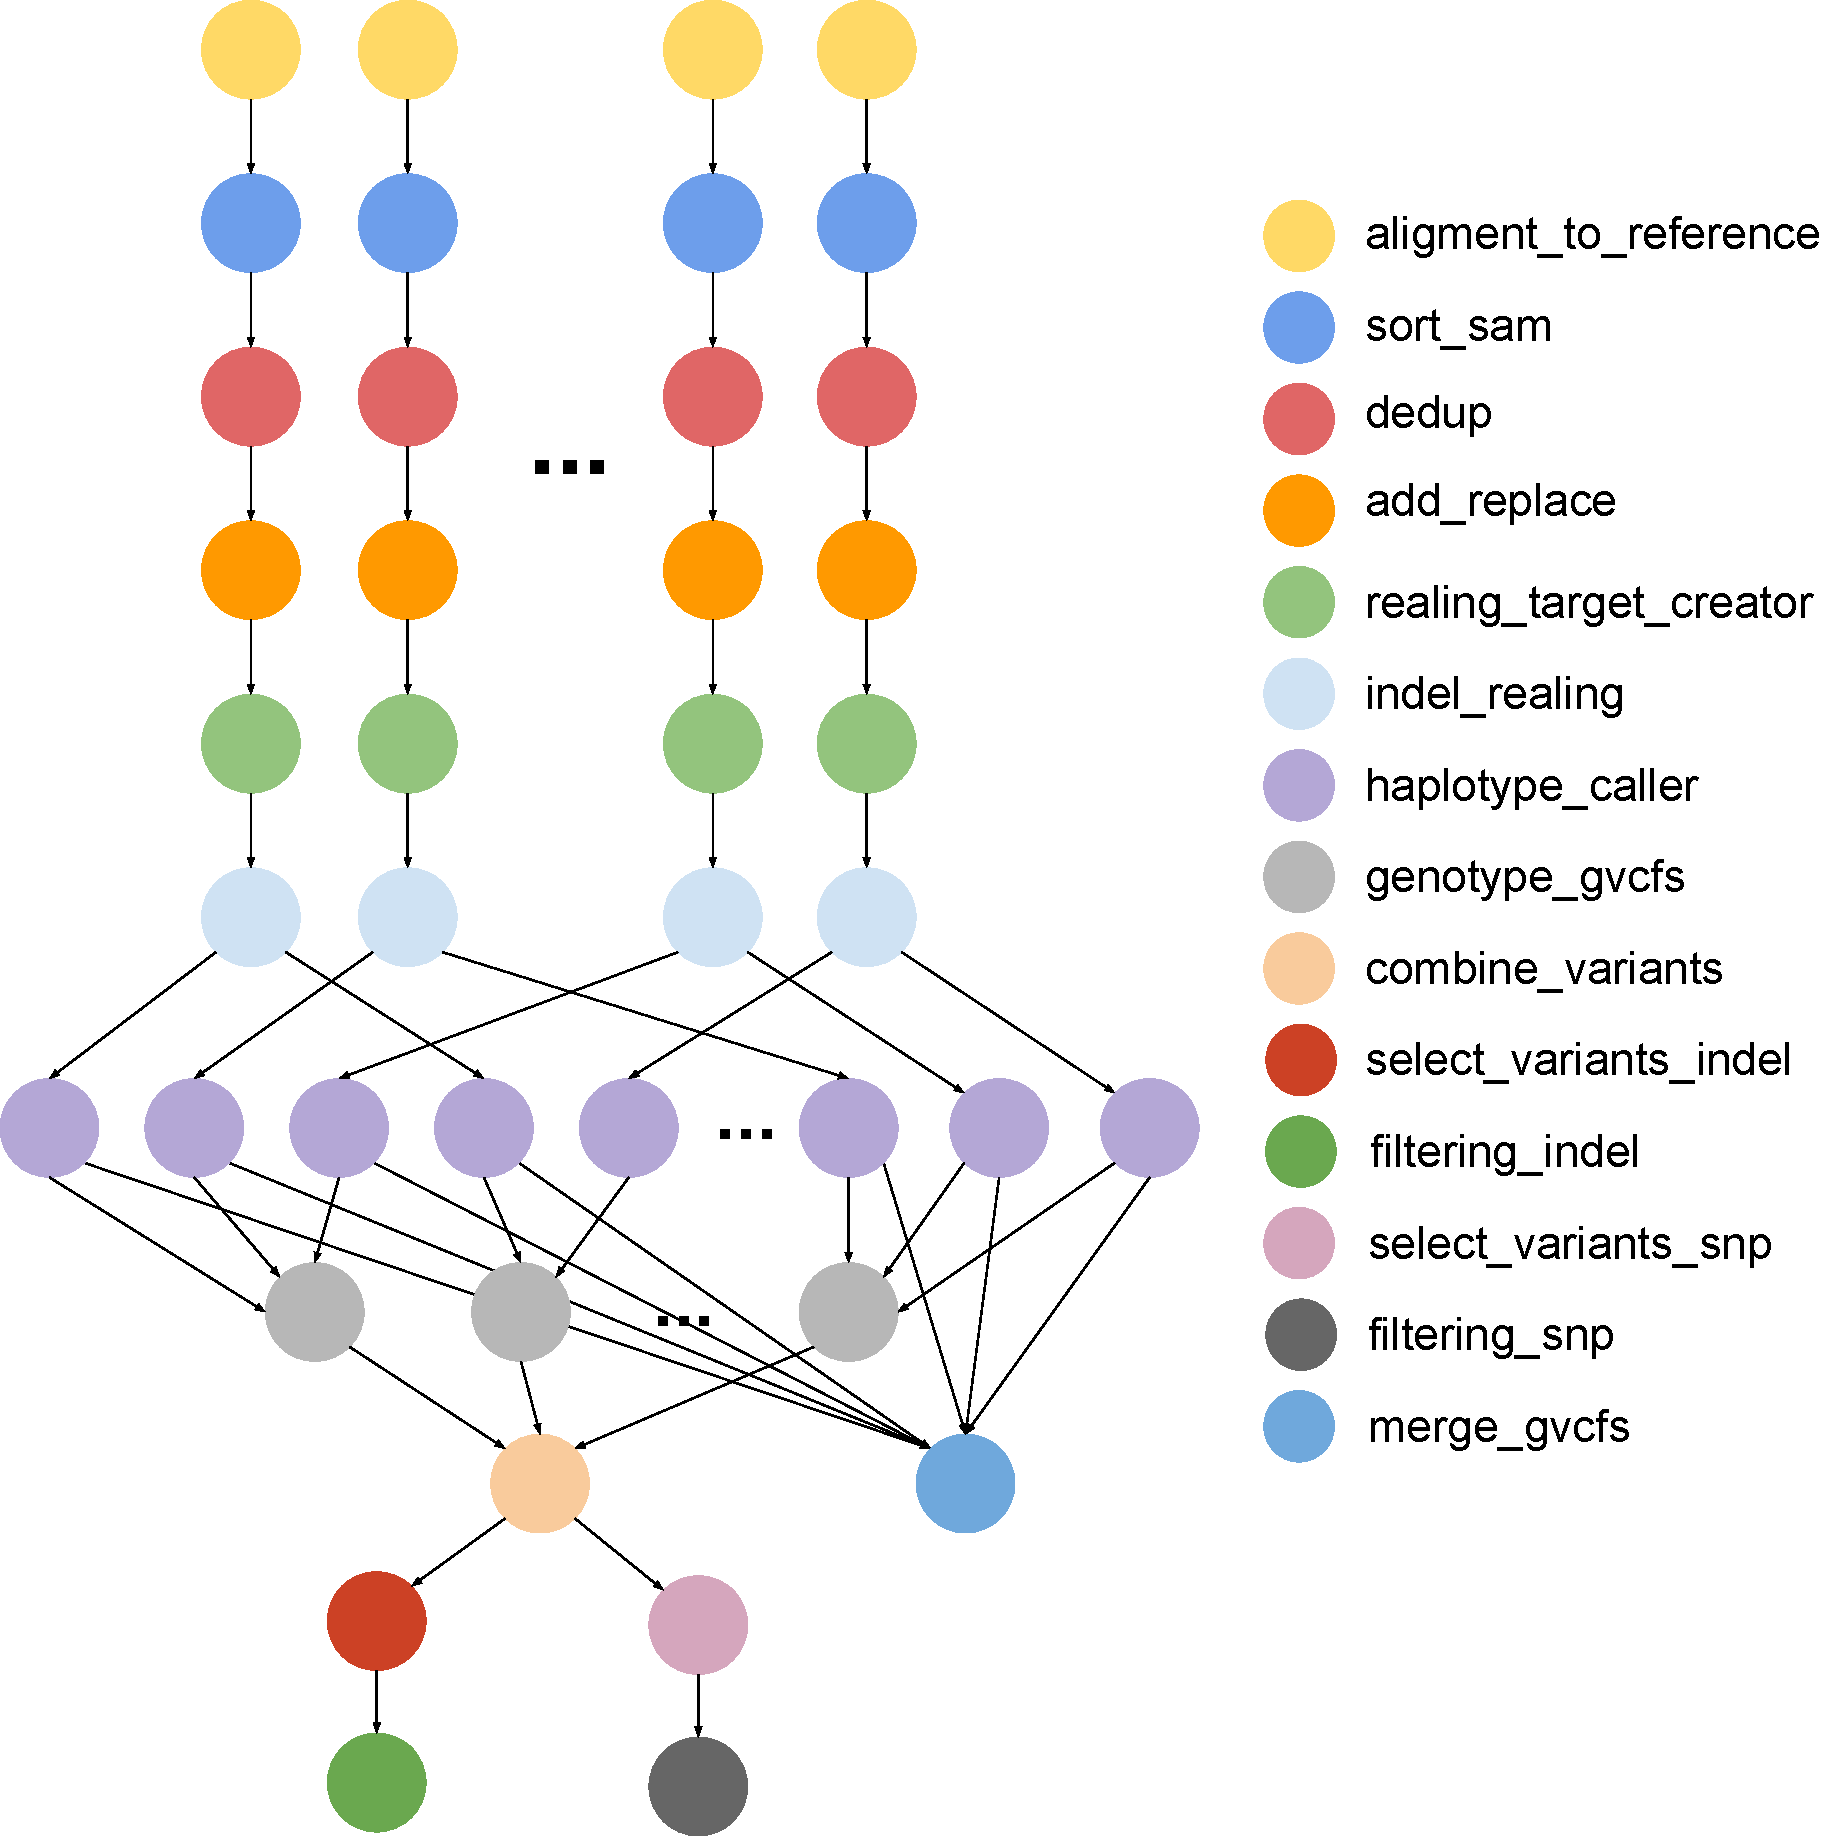
\includegraphics[width=0.95\linewidth]{figures/workflow-soybean}
	\caption{SoyKB workflow.}
	\label{fig:workflow-soykb}
\end{figure}


% Generating Semantic Annotations
\subsubsection{Generating Semantic Annotations}
Figure~\ref{fig:annotations} shows a simplified overview of the annotations generated for the Montage workflow using the WICUS ontology network.

\begin{figure}[!htb]
	\centering
	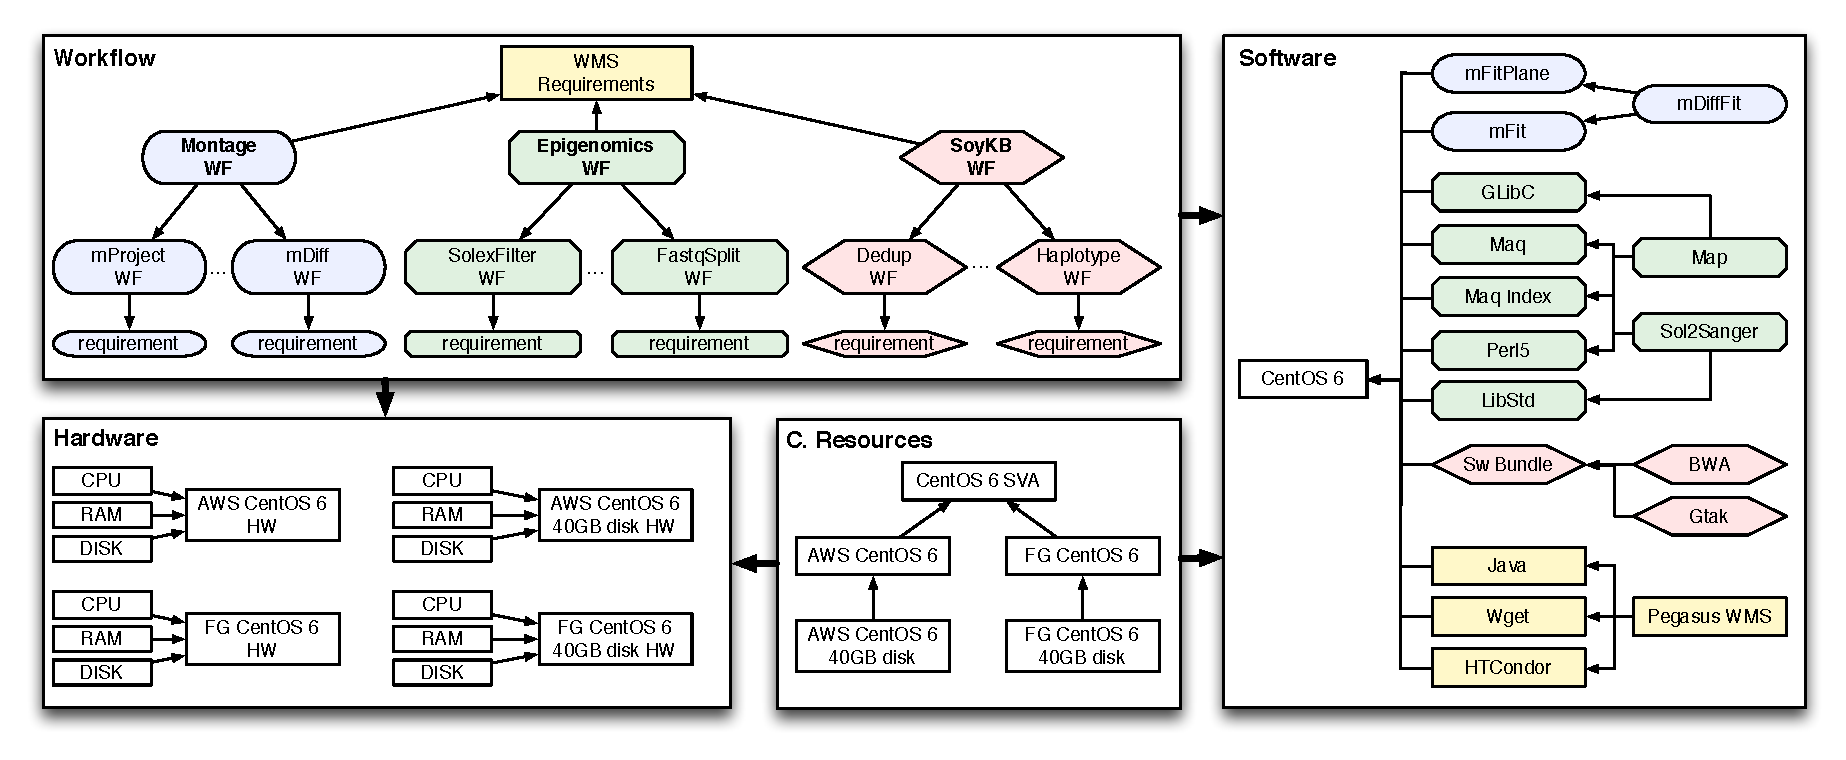
\includegraphics[width=\linewidth]{figures/annotations}
	\caption{Annotations for the Montage workflow using the WICUS ontology network.}
	\label{fig:annotations}
\end{figure}

 As shown in Figure~\ref{fig:wicusflow}, the first step in the process of documenting a workflow is the annotation of the workflow DAX file. We use the \texttt{Workflow} domain ontology to describe the Montage workflow as 1) an individual that represents the top level workflow, and 2) another 9 individuals representing its sub-workflows, one for each transformation. We also generate 10 requirements, one for the top level workflow, which specifies the WMS requirements, and the remaining for defining the software components required by each transformation. At this point, these requirements are empty, as they are not yet related to their software components.
 
In this experiment, we address two types of components: the WMS and the application related components. The WMS components include the workflow engine, in our case the Pegasus WMS, and its dependencies. Pegasus uses HTCondor as task manager, and also depends on Java. We use the \texttt{Software} domain ontology to describe these components as individuals, and to represent their dependencies. The 3 components also depend on the operating system, which in our case is CentOS.

To describe the deployment of the WMS components, we studied their installation processes according to their documentation. We then defined a set of installation bash scripts for each of them. These scripts are included on the deployment plans of the components along with their configuration information.  
 
Application components are described from the Montage workflow's Transformation Catalog, where the binary file, version, and destination path are defined. These components are also described as individuals using the \texttt{Software} domain ontology. We use this information to generate the configuration parameters of the deployment script, which in this case is the same for all components. The script downloads the binary files from an online repository and copies them to the specified destination path. This process identified 59 software components for the Montage workflow that are annotated and included in the Software Components Catalog.
Then, the Transformation Catalog Annotator module relates each transformation requirement, defined using the \texttt{Workflow} domain ontology, to the application component, and therefore to the deployment information.
In this experiment, we define 9 Montage components that are linked to the requirements, and another two sub-components that are defined as dependencies in the software catalog (\emph{mDiffFit} depends on the \emph{mDiff} and \emph{mFitPlane} components).

To describe computational resources we use the \texttt{Computing Resources} and \texttt{Hardware} domain ontologies. The Scientific Virtual Appliances Catalog includes the description of two virtual machine images, one for FutureGrid and another for Amazon EC2. These two images are conceptually equivalent, as they both provide CentOS 6 operating system.
Therefore, we generate two Image Appliances (FG CentOS 6 and AWS CentOS 6) that are grouped into one single Scientific Virtual Appliance (CentOS 6 SVA). Depending on which providers are available, one or the other will be selected.


\subsubsection{Reproducing Workflow Executions.}

The last step on the process for achieving reproducibility in scientific workflows (Figure~\ref{fig:wicusflow}) is to execute the Infrastructure Specification Algorithm (ISA). The ISA combines the annotated data based on the 4 domain ontologies in order to find a suitable infrastructure specification that is able to run the workflow. The algorithm retrieves and propagates the WMS requirements of the top-level workflow (\texttt{Workflow} domain ontology) to its related sub-workflows. Requirements and software components are matched, and a dependency graph is built based on the relation between the requirements and the component dependencies. This graph is then used to compute the intersection between the set of software components from the SVA and the dependency graph of each sub-workflow. ISA selects the intersection where the value is maximized for each sub-workflow. Software components already available in the SVA are then removed from the chosen graph. To reduce the number of SVAs, the algorithm attempts to merge sub-workflows requirements into a single SVA. Requirements can be merged if all their software components are compatible. Finally, ISA generates a PRECIP script with the set of required instructions to instantiate, configure, and deploy the computational resources and software components.


In this experiment, we execute ISA over the annotated data in a scenario where FutureGrid is the only available platform for resource provisioning, and in a scenario where the available platform is Amazon EC2. In both cases, the algorithm is able to obtain a PRECIP script for each infrastructure. Each generated script is composed by the following main sections:

\begin{itemize}

	\item \emph{Experiment Creation}: generates a new experiment using the given VM image ID and the user credentials for the selected infrastructure provider;
    	    
	\item \emph{Software Deployment}: executes the set of instructions defined on the deployment plan of each software component to install and configure the required software to execute the workflow. In this section, both the workflow management system and the application are deployed with their dependencies;

	\item \emph{User Setup}: creates a user account on the VM (if it does not exist) and configures the necessary SSH keys to enable file transfers and execution. This account will be used to run the workflow;
	   
	\item \emph{Data Stage and Workflow Execution}: stages all the input data of the Montage workflow on the VM, and launches the workflow execution. Since our work is focused on infrastructure reproducibility, data and workflow management are not covered in our approach.

\end{itemize}

\noindent Note that all the configuration and deployment commands (first 3 sections) require superuser privileges on the VM. The workflow execution, however, is performed under the user account created in the third section.

We executed the scripts on their corresponding platforms. Both executions succeeded on deploying and running the Montage workflow, the Pegasus WMS, and their dependencies. We also performed the same execution of the Montage workflow in a predefined VM image, where the execution environment is already in place. Results show that the VM execution environments deployed by both scripts are equivalent to the former one. In addition, we used a perceptual hash tool\footnote{pHash - \url{http://www.phash.org}} to compare the resulting image (0.1 degree image of the sky) generated by both executions against the one generated by the baseline execution. We obtained a similarity factor of 1.0 (over 1.0) with a threshold of 0.85, which means the images are identical. Therefore we are obtaining the same results as the original workflow. In this work we do not aim to reproduce either the performance or the execution time of the original experiment.


All the original and generated scripts are available as part of the experimental material included in the Research Object (RO)~\cite{researchObjects} associated with this paper\footnote{\url{http://pegasus.isi.edu/publications/reppar}}. This RO also contains pointers to the software and resources used in this experiment.



% Section
\section{Related Work}
\label{sec:related-work}

A computational experiment involves several elements that must be conserved to ensure reproducibility. Most of the works addresses the conservation of data and the workflow description, however the computational environment is often neglected. 
An study to evaluate reproducibility in scientific workflows is conducted in~\cite{zhao2012}. The study evaluates a set of domain-specific workflows, available in the myExperiment~\cite{myExperiment} collaborative environment, to identify causes of workflow decays. The study shows that nearly 80\% of the workflows cannot be reproduced, and that about 12\% are due to the lack of information about the execution environment, and that 50\% are due to the use of third-party resources such as web services and databases. Note that some of those third-party resource issues could be also considered as execution environment problems. 

The Executable Paper Grand Challenge~\cite{elsevierchallenge} and the SIGMOD conference in 2011~\cite{SIGMOD} highlighted the importance of allowing the scientific community to reexamine an experiment execution. The conservation of virtual machine (VM) images emerges as a way of preserving the execution environment~\cite{Brammer,SHARE}. However, the high storage demand of VM images remains a challenging problem~\cite{Mao:2014:ROD:2600090.2512348,6552826}. Moreover, the cost of storing and managing data in the Cloud is still high, and the execution of high-interactivity experiments through a network connection to remote virtual machines is also challenging. A list of advantages and challenges of using VMs for achieving reproducibility is exposed in~\cite{Howe2012}. ReproZip~\cite{reprozip} is a provenance-based tool that tracks operating system calls to identify the libraries and data dependencies, as well as the configuration parameters involved in an experiment. The tool combines all these dependencies into a single package that can be used to reproduce an experiment. Although this approach avoids storing VM images, it still requires storing the application binaries and their dependencies. Instead, our work uses semantic annotations to describe these dependencies.

Software components cannot be preserved just by maintaining their binary executable code, but by guaranteeing the performance of their features. In~\cite{Matthews}, the concept of adequacy is introduced to measure how a software component behaves relatively to a certain set of features. Our work is based on this same concept, where we build a conceptual model to semantically annotate the relevant properties of each software component. Then, we use scripting to reconstruct an equivalent computational environment using these annotations.

A recent and relevant contribution to the state of the art of workflow preservation is being developed within the context of the TIMBUS project~\cite{timbus}. The project  aims to preserve and ensure the availability of business processes and their computational infrastructure, aligned with the enterprise risk and the business continuity managements. They also propose a semantic approach for describing the execution environment of a process.  Even though TIMBUS has studied the applicability of their approach to the eScience domain, their approach is mainly focused on business processes.


% Section
\section{Conclusion and Future Work}
\label{sec:conclusion}

In this work, we proposed a semantic modeling approach to conserve computational environments in scientific workflow executions, where  the resources involved in the execution of the experiment are described using a set of semantic vocabularies. We defined and implemented 4 domain ontologies, aggregated in the the WICUS ontology network. From these models, we defined a process for documenting a workflow application (Montage), a workflow management system (the Pegasus WMS), and their dependencies. We then used the PRECIP experiment management tool to describe and execute the experiment. Experimental results show that our approach can reproduce an equivalent execution environment of a predefined VM image on an academic and a public Cloud platforms.

The semantic annotations of the computational environment combined with the scripting functionality provided by PRECIP is a powerful approach for achieving reproducibility of computational environments in future experiments, and at the same time addresses the challenges of high storage demand of VM images. The drawback of our approach is that it assumes the application and the workflow management system binaries are publicly available.

In the future we plan to apply our approach in a larger set of scientific workflows and involve users from different scientific areas, aiming to automate the generation process of the semantic annotations to describe both the workflow application and the workflow management system. We also plan to extend the WICUS ontology network to include new concepts and relations such as software variants, incompatibilities, and user policies for resource consumption.



% Acknowledgements
\section*{Acknowledgements}

This material is based upon work supported in part by the National Science Foundation under Grant No. 0910812 to Indiana University for ``FutureGrid: An Experimental, High-Performance Grid Test-bed'', the FPU grant from the Spanish Science and Innovation Ministry (MICINN), and the Ministerio de Econom\'ia y Competitividad (Spain) project "4V: Volumen, Velocidad, Variedad y Validez en la Gesti\'on Innovadora de Datos" (TIN2013-46238-C4-2-R). We also thank Gideon Juve and Karan Vahi for their valuable help.


% Bibliography
\bibliographystyle{elsarticle-num}
\bibliography{references}

\end{document}